%%%%%%%%%%%%%%%%%%%[ INTRODUCTION ]%%%%%%%%%%%%%%%%
\addtocontents{toc}{\cftpagenumbersoff{chapter}}
\setstretch{2}

\chapter[INTRODUCTION]{\fontsize{16}{12}\vspace{-.59in}\selectfont INTRODUCTION}

\pagenumbering{arabic}

%\section[General Background]{\fontsize{14}{12}\selectfont \MakeUppercase{GENERAL BACKGROUND}}


\label{Intro}
\newline
\paragraph{}
 In the rapidly evolving landscape of education, the need for innovative and data-driven methods to assess and enhance students' academic performance has become more pronounced. This project aims to revolutionize the traditional methods of evaluating students by leveraging the power of Natural Language Processing (NLP) and Deep Learning in the context of live classroom interactions. Recognizing the evolving nature of learning, this project aims to shift the paradigm of academic assessment by integrating cutting-edge technologies. The model focuses on analyzing live classroom interactions to provide a real-time and comprehensive evaluation of students' academic performance. Through this approach, the model seeks to enhance the traditional methods of assessment by incorporating dynamic feedback mechanisms, sentiment analysis, and personalized learning paths. 
\par The core objectives of this model encompass the establishment of a real-time feedback mechanism, employing NLP algorithms to assess communication skills, engagement, and content comprehension. Sentiment analysis is employed to discern the emotional undertones during live interactions, correlating these sentiments with academic performance. Deep learning models are applied to recognize individual learning paths based on students' strengths and weaknesses, fostering adaptive recommendations. Furthermore, the model aims to quantify and integrate participation metrics into the overall academic evaluation, acknowledging the importance of collaborative engagement.
\par This model holds significant implications for the future of education. By embracing NLP and Deep Learning, it endeavors to provide educators with valuable insights into students' understanding, participation, and emotional engagement during live classroom sessions. The dynamic nature of the assessment allows for personalized learning experiences, catering to individual needs and learning styles. Beyond immediate applications, the model contributes to the broader discourse on data-driven, interactive, and adaptive learning methodologies. Its findings may pave the way for transformative shifts in educational practices, promoting a more responsive and engaging approach to student evaluation.


%%%%%%%%%%%%%%%%[ LITERATURE SURVEY ]%%%%%%%%%%%%%%%%

\chapter[LITERATURE SURVEY]{\fontsize{16}{12}\vspace{-.59in}\selectfont LITERATURE SURVEY}
%Give a detailed description of the literature review. Give appropriate citations. Each paper can be given a separate section\\


\paragraph{}
In the paper by  Zhen et al.[1], the research investigates the link between classroom dialogue and academic performance in primary school, employing text classification models for interaction feature identification. It successfully overcomes challenges in analyzing large-scale text data by using the BERT model for recognizing emotional expression and interactive types. The findings emphasize the importance of interactive types, highlighting their superior predictive power over emotional expression in both non-STEM and STEM courses, with nuanced effects observed across different stages of the class for each course type.
\par The system proposed by Gupta et al.[2] suggests a deep learning-based method using facial emotions to gauge real-time engagement of online learners, aiming to replicate traditional classroom interaction. The study evaluates models like Inception-V3, VGG19, and ResNet-50, finding that ResNet-50 performs best with a 92.3\% accuracy in classifying facial emotions during online learning sessions. The proposed system exhibits promising results in enhancing the interactivity of online education through real-time engagement detection.
\par Fahd et al.[3] introduces a novel approach utilizing machine learning models on publicly available datasets related to student interactions with learning management systems in blended learning environments. The focus is on identifying students at risk of failing, aiming for timely intervention to enhance academic progress. The chosen machine learning algorithm, random forest, achieves an 85\% accuracy, offering a promising tool for educators to implement targeted pedagogical practices and support students' learning effectively.
\par A novel sentiment analysis approach using a Bayesian CNN-LSTM model was proposed by Mrhar et al.[4] to analyze social interactions in Massive Open Online Courses (MOOCs). By leveraging deep learning architectures and quantifying uncertainty with a Bayesian neural network, the model demonstrates promising performance in accuracy, precision, recall, and F1-Score compared to other models (CNN-LSTM, CNN, LSTM). The study reveals a significant correlation between sentiment in forum posts and the dropout rate in MOOCs, highlighting the potential for personalized interventions to enhance learner engagement and course effectiveness.
\par The paper by Nezami et al.[5] introduced a two-step deep learning model for engagement recognition from images, addressing the challenge of limited data by pre-training on facial expression data. The first step involves training a facial expression recognition model, and in the second step, the model's weights initialize the engagement recognition model. The proposed engagement model, trained on a new dataset with 4627 samples, outperforms other deep learning architectures, including those applied for the first time to engagement recognition, as well as methods using histogram of oriented gradients and support vector machine.
\par Alyuz et al.[6] conducted a longitudinal research addresses the limitation of existing Intelligent Tutoring Systems (ITSs) in accurately tracking learners' affective states, crucial for a personalized learning experience. By collecting data from authentic classroom pilots through appearance and context-performance modalities, the study focuses on detecting learning-related states such as 'Satisfied,' 'Bored,' and 'Confused.' The proposed hierarchical semi-supervised model adaptation method achieves highly accurate emotional engagement detection, with an 89.23\% and 75.20\% F1 measure for the instructional and assessment sections, respectively, showcasing the effectiveness of personalized emotional engagement detectors.
\par In the paper, Nigel Bosch [7] underscores the importance of engagement in learning and explores the potential of computerized learning environments to enhance the student experience by automatically detecting engagement and disengagement. Building upon previous studies that utilized facial features for automatic engagement detection, the research proposes new methods, including third-party observer annotations for comparison and the improvement of automatic detectors through feature engineering. The study aims to refine the accuracy of engagement classification based on facial expressions, offering insights into optimizing adaptive learning environments for students.
\par In the paper, Bosch et al.[8] proposes computer vision and machine-learning techniques to detect students' affect from facial expressions and gross body movements during interactions with an educational physics game. The research, conducted in a real-world school computer lab with up to 30 students, demonstrates promising results in cross-validated classification accuracies for various affective states, including boredom, confusion, delight, engagement, frustration, and off-task behavior. The findings suggest the feasibility and generalizability of video-based detectors for naturalistic affect in educational settings, paving the way for affect-sensitive interventions in intelligent educational interfaces and games.
\par Blanchard et al.[9] proposes a method to detect mind wandering during learning by monitoring physiological measures such as skin conductance and temperature. In a study on students learning research methods, supervised classification models achieved a kappa value of 0.22, indicating feasibility for student-independent mind-wandering detection. Despite modest accuracy, these results mark a significant step towards developing fully automated and unobtrusive methods for identifying mind wandering during the learning process.
\par In the paper, Monkaresi et al.[10] investigated the use of computer vision techniques to detect engagement in 22 students during a structured writing activity. Using features extracted from videos, including heart rate and facial animation units, the supervised learning approach achieved promising results with an Area under the ROC Curve (AUC) of 0.758 for concurrent engagement annotations and 0.733 for retrospective annotations. The fusion of channels, including Kinect Face Tracker features, demonstrated the best overall performance.
\par A paper by Whitehill et al.[11] proposed an automatic recognition of student engagement through facial expressions, comparing human observers' judgments with machine learning-based automated detectors. The study reveals that human observers reliably discriminate between low and high degrees of engagement, with a high agreement. Automated detectors for binary classification demonstrate comparable accuracy to humans, and both human and automatic engagement judgments correlate with student task performance, suggesting the potential for leveraging facial expressions as an indicator of student engagement in educational settings.
\par Baker et al.[12] investigated off-task behavior, specifically focusing on "gaming the system," in classrooms using intelligent tutoring software. The research reveals that gaming the system is strongly associated with reduced learning, with a student's frequency of this behavior correlating as strongly to post-test scores as their prior domain knowledge and academic achievement.




%%%%%%%%%%%%%%%%%%%[(Base Paper) ]%%%%%%%%%%%%%%%%%%%

\chapter[SYSTEM ANALYSIS]{\fontsize{16}{12}\vspace{-.59in}\selectfont SYSTEM ANALYSIS}
\section{Existing System}
\paragraph{}
The current system for predicting the academic performance of students in live classroom interactions is a multifaceted approach that incorporates both traditional assessment methods and qualitative observations. Traditional grading methods, including exams, quizzes, assignments, and projects, serve as a foundational aspect, providing a quantitative measure of a student's understanding of the material. 
\par Beyond these quantitative measures, teachers actively observe and evaluate students based on their participation and engagement during live classroom interactions. This involves assessing students' abilities to ask and answer questions, contribute to discussions, and be actively involved in class activities. Additionally, attendance is closely monitored, as consistent presence in class is often correlated with improved academic performance. The completion of homework and assignments is considered as it reflects a student's effort, understanding, and application of the concepts covered in class. Formative assessments, such as quizzes or short tests, are periodically conducted to gauge ongoing understanding and identify areas that may need additional attention. 
\par Teacher feedback, provided qualitatively, offers insights into students' strengths, weaknesses, and recommendations for improvement. Classroom interactions and discussions are observed to understand how well students comprehend and articulate concepts, involving verbal communication and participation in group activities. Parent-teacher meetings provide an additional channel for discussing a student's academic progress, behavior, and areas for improvement. 
\par Moreover, some educational institutions may integrate technological tools, such as Learning Management Systems (LMS) or online platforms, to track and analyze student performance data. Historical performance, including previous academic records and performance in earlier grades or courses, is often considered to assess a student's overall academic history. While the existing system provides a comprehensive overview, there is a growing trend towards incorporating more data-driven and technology-based approaches to enhance the accuracy and efficiency of performance predictions in the educational landscape.
\section{Proposed System}
\paragraph{}
By embracing machine learning algorithms, the system seeks to analyze an extensive array of data points, encompassing conventional metrics like grades and attendance records alongside more nuanced indicators such as participation levels and real-time engagement during live classroom interactions. The incorporation of smart classroom technologies and online platforms enables the real-time tracking of student activities, providing a dynamic understanding of their learning behaviors.
\par Natural Language Processing (NLP) techniques are envisaged to play a pivotal role in evaluating the content of students' interactions, shedding light on their comprehension, critical thinking skills, and overall proficiency in the subject matter. Additionally, sentiment analysis tools will be deployed to discern the emotional tone and sentiment expressed by students during interactions, offering valuable insights into their learning experiences. 
\par The proposed system for predicting the academic performance of students in live classroom interactions represents a forward-looking paradigm that harnesses the power of advanced technologies and data analytics to revolutionize the traditional assessment methodologies. The system advocates for continuous communication channels, facilitated through digital platforms, to establish regular feedback loops among teachers, students, and parents. This collaborative and technologically-driven approach reflects the evolving landscape of education, emphasizing the need for tailored and data-informed strategies to optimize the learning journey and enhance overall academic outcomes. It involves several steps leveraging advanced technologies and data analytics. 
\\
1) Data Collection
\\
2) Data Preprocessing
\\
3) Machine Learning Model Selection
\\
4) Training the Model
\\
5) Real-Time Data Integration
\\
6) Sentiment Analysis
\\
7) Model Evaluation
\\
8) Deployment
\\
9) Communication and Reporting

\section{Objectives of Proposed System}
\begin{itemize}
   \item Improve the accuracy of predicting academic performance using advanced algorithms for more reliable assessments.
    \item Assess students' engagement and sentiments in real-time during live classes to provide instant insights and timely interventions.
    \item Consider a mix of traditional and dynamic indicators to create a complete view of students' academic performance beyond just grades.
    \item Provide personalized feedback to students, educators, and parents based on real-time assessments, tailored to individual learning needs.
    \item Continuously improve the prediction model by learning from new data and adjusting predictions over time based on feedback.
    \item Seamlessly integrate with smart classroom technologies and online platforms to enhance data collection and real-time monitoring.
    \item Establish clear communication channels among educators, students, and parents for transparent reporting of predicted academic performance.
    \item Identify and address potential challenges early on to create an environment that supports student success and well-being.
    \item Encourage data-driven decision-making in education by providing actionable insights for educators and administrators.
    \item Ensure the ethical use of data, privacy considerations, and transparency in applying predictive analytics for academic performance.
\end{itemize}

\subsection{Advantages of Proposed System}
\begin{itemize}
\item Better Accuracy: The system uses advanced tools for more accurate predictions of how students will perform academically, offering reliable insights.
\item Quick Support: Educators can step in quickly to help students when needed, thanks to the system's ability to assess and address issues in real-time during live classes.
\item Personalized Feedback: The system provides specific and personalized feedback to each student, educator, and parent based on real-time assessments, offering individualized insights.
\item Optimized Learning: Early problem spotting and timely interventions create an environment that supports student success and well-being, contributing to an enhanced learning experience..
\item Effective Communication: Open and effective communication channels between educators, students, and parents are promoted, fostering transparency and collaboration.
\item Tech Integration: The system easily integrates with smart classroom technologies and online platforms, making data collection and monitoring efficient and compatible.
\item Ethical Approach: Ethical standards and privacy considerations are prioritized in the use of predictive analytics, ensuring responsible and transparent handling of student data.






\end{itemize}

\section{User Requirement Specification}
\paragraph{}
The User Requirement Specification for the proposed academic performance prediction system outlines key functionalities. It covers user profiles for administrators, educators, students, and parents, specifying real-time assessments, predictive analytics, personalized feedback, and secure data handling. The system should feature a user-friendly interface, integrate with existing systems, facilitate effective communication, and ensure continuous improvement. Ethical considerations, scalability, and user training are emphasized. This concise document serves as a guide for developing a comprehensive and user-centric educational technology solution.

\begin{itemize}
    \item Functional Requirements
    \begin{enumerate}
      \item The system should have a secure user authentication mechanism for educators, students, and parents, ensuring access control and data privacy. It must collect a diverse range of data, including grades, attendance records, live classroom interactions, and participation levels.
    \item The system should provide real-time assessment capabilities during live classroom interactions, including monitoring participation, engagement, and sentiment analysis.
    \item It should implement machine learning algorithms to create a prediction model capable of accurately forecasting academic performance based on collected data.
    \item Generate and deliver personalized feedback to students, educators, and parents, offering insights and recommendations tailored to individual learning needs.
    \item Design the system for continuous learning, allowing it to adapt to new data and improve its predictive capabilities over time.
    \item Seamlessly integrate with smart classroom technologies and online platforms to enhance data collection, storage, and real-time monitoring.
    \end{enumerate}
\end{itemize}

\begin{itemize}
    \item Non Functional Requirements
    \begin{enumerate}
        \item The system must prioritize security measures to protect user data, including encryption, secure connections, and secure user authentication.
    \item Design the system to handle a scalable number of users, accommodating growth in user base and data volume.
    \item Ensure the system's performance is optimized for real-time assessment, with minimal latency in processing and delivering predictions.
    \item Guarantee the reliability of the system, minimizing downtime and ensuring consistent availability during live classroom interactions.
    \item Set high standards for the accuracy of predictions, regularly evaluating and refining the machine learning model for optimal performance.
    \item Ensure the system is accessible to users with diverse abilities, incorporating features that support accessibility standards.
    \end{enumerate}
\end{itemize}

\section{Feasibility Study}
\paragraph{}
The feasibility study aims to assess the viability of implementing an advanced system that leverages technology for real-time assessments and predictions. This study encompasses technical, economic, and operational perspectives to guide decision-making. Following are the
feasibility study employed,
\begin{itemize}
\item Technical Feasibility
\item Economic Feasibility
\item Operational Feasibility
\end{itemize}

\subsection {Technical Feasibility}
\par \hspace{1cm}Technical feasibility assesses whether the proposed system can be successfully developed and implemented from a technological standpoint. In the context of the Academic Performance Prediction System in Live Classroom Interactions, several key aspects contribute to its technical feasibility:
\begin{itemize}
\item System Architecture: Ensure the system easily fits with existing technologies and can grow as more users join.
\item Machine Learning Algorithms: Advanced machine learning algorithms are fundamental for predictive analysis. The technical feasibility depends on selecting and implementing algorithms capable of handling real-time data during live classroom interactions and adapting to continuous learning.
\item Data Security and Privacy: Keep student info safe by using strong encryption and controls against unauthorized access.
\item Integration with Existing Technologies: Connect smoothly with current smart classroom tools and online platforms for easy data sharing.
\item User Interface and Experience: Design an easy-to-use interface that makes sense for educators, students, and parents.
\end{itemize}
\subsection {Economic Feasibility}
\par \hspace{1cm}Economic feasibility is a crucial aspect of any proposed project, including the development and implementation of the Academic Performance Prediction System in Live Classroom Interactions. It involves evaluating the financial viability of the project throughout its lifecycle, from initial development costs to ongoing operational expenses. The following are the key considerations for economic feasibility:
\begin{itemize}
\item Cost of Development: Expenses for creating the system, including developer salaries, software/hardware costs, and third-party services.
\item Operational Costs: Ongoing expenses after development, like maintenance, hosting, user support, and training
\item Return on Investment (ROI): Comparing expected benefits (better grades, improved communication) against total costs. Deciding if the investment will bring positive returns.
\end{itemize}
\subsection {Operational Feasibility}
\par \hspace{1cm}Operational feasibility assesses the practicality of implementing a proposed system within the existing organizational context. It focuses on whether the system can be smoothly integrated into current practices and processes, and if users can adapt to and effectively use the new system. The following are key aspects of operational feasibility:
\begin{itemize}
\item User Acceptance: Check if users (educators, students, and parents) are willing and ready to accept the new system.
\item Integration with Current Practices: Ensure the new system fits well with existing educational processes to minimize disruptions.
\item Stakeholder Involvement: Involve educators, students, parents, and administrators in planning to meet diverse needs.
\item User Satisfaction: Aim for a system that meets user expectations, is user-friendly, and enhances the overall educational experience.
\end{itemize}
\section{System Specification}
\paragraph{}
A system requirements specification is a structured collection of information that represents the requirements of a system. Non functional requirements do impose constraints on the design or implementation( such as performance quality standards engineering requirements or design constraints). The system leverages advanced technologies, including machine learning algorithms and smart classroom integration, to offer accurate insights into students' academic performance. The software requirements specification lists all necessary requirements if met will offer better optimum software usability.

The system requirements of the project include
\begin{itemize}
    \item Software specification
    \item Hardware specification
\end{itemize}

\subsection{Hardware specification}
\paragraph{}
For optimal performance, it is advisable to have the following minimum hardware specifications installed on both the server hosting the Academic Performance Prediction System and the client devices accessing the system.
\begin{itemize}
    \item PROCESSOR : 64bit
    \item RAM : Min 8GB
    \item HARD DISK : 256 GB SSD or higher
\end{itemize}

\subsection{Software specification}
\paragraph{}
For the proposed system to work properly, it is necessary that following software are installed and running on the server / client.
\begin{itemize}
    \item Operating system : Windows, macOS, and Linux
    \item Language Used : Python
    \item Database : MYSQL
    \item Framework : Django and Mediapipe
    \item IDE : Visual Studio Code, PyCharm or Collab
\end{itemize}

\chapter[DESIGN AND DEVELOPMENT]{\fontsize{16}{12}\vspace{-.59in}\selectfont DESIGN AND DEVELOPMENT}

\section{Methodology}
Methodology comprises four key steps:
\begin{itemize}
    \item Data collection
    \item Data preprocessing
    \item Model training
    \item Model evaluation
\end{itemize}
\par First, data was collected from live classroom interactions, followed by preprocessing to refine the dataset. Next, a Convolutional Neural Network (CNN) model is trained to classify dialogues and predict academic performance. Finally, the model is evaluated to gauge its accuracy and efficiency in predicting academic outcomes.

The study uses the FER-2013 dataset, containing around 30,000 grayscale facial images depicting various expressions. It includes 28,709 training examples and 3,589 test examples, with labels representing seven emotions: 
\begin{itemize}
    \item 0=Angry
    \item 1=Disgust
    \item 2=Fear
    \item 3=Happy
    \item 4=Sad
    \item 5=Surprise
    \item 6=Neutral
\end{itemize}


\par Data preprocessing is essential for training it includes segregating data, extracting and reshaping pixel values into a 4D NumPy array, normalizing them, and OneHotEncoding categorical values into binary. Finally, the processed data is converted into a NumPy array for compatibility with machine learning libraries.

\par A CNN model with Conv2D, BatchNormalization, ReLU activation, MaxPooling2D, Dropout layers, and a Flatten layer is utilised.

\par The prediction of academic performance are made from facial expression, body posture analysis and sentiment analysis from the remarks in assigned works for the student.
\begin{figure}[!ht]
\centering
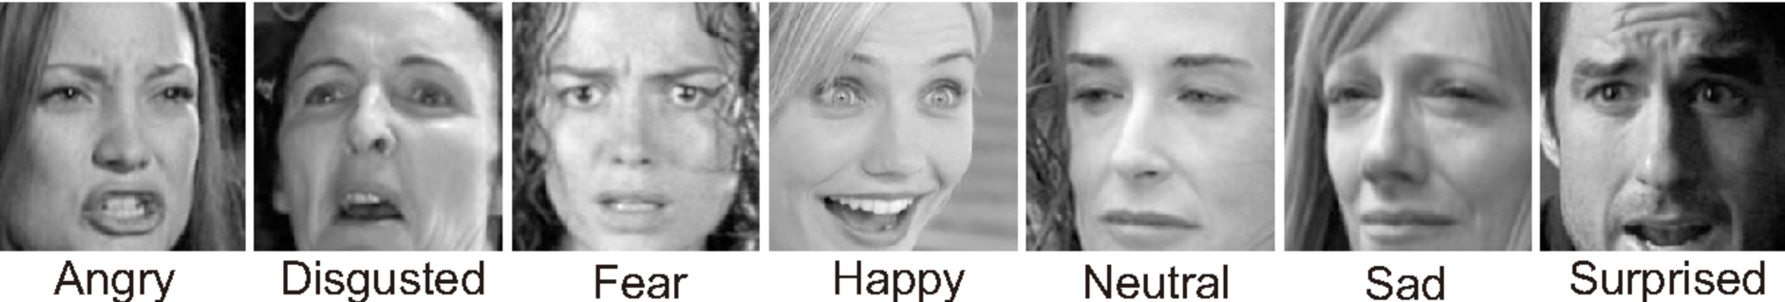
\includegraphics[width=125mm]{dataset-cover.png}
\caption{Samples of FER-2013}
\end{figure} 

\section{Users of the system}
\begin{itemize}
    \item Admin
    \item Staff
    \item Student
\end{itemize}

\section{Modules}
\subsection{Functions Of Admin}
\begin{itemize}
    \item Add and manage course
    \item Add and manage subject 
    \item Add and manage staff
    \item Subject allocation to staff
    \item View Student Performance
    \item View Complaints 
    
\end{itemize}
\par Admin controls staff and students. Admin can add and manage new staff, subject and course. It can also view complaints, the respective reply and student performance.

\subsection{Functions Of Staff}
\begin{itemize}
    \item Add and manage study Material 
    \item Add Assignments
    \item View allocated subjects 
    \item View and remark assignment
    \item View Student Performance
    \item View and reply Complaints 
    \item View feedback
\end{itemize}
\par Staff can add new study materials, reply for the complaint. It can also view the feedback, Student performance and allocated subjects. And also add new assignments, view work and add remarks for works.

\subsection{Functions Of Student}
\begin{itemize}
    \item View study Material 
    \item View subjects 
    \item View and upload Assignment
    \item View Student Performance
    \item Add Complaints and view reply
    \item Add feedback
\end{itemize}
\par Student can submit complaint on particular staff and feedback on particular subject. It can also view study materials uploaded by staff, subjects and student performance. And can view work assigned and can upload it.


\section{System Architecture}
\par \hspace{1cm}The proposed design mentioned in the document consists of several components. The first component is a CNN model that is used for image training. This model is implemented using TensorFlow and deployed using Keras. OpenCV is used for image processing.
The second component is the interface of the system. The front-end of the interface is created using HTML, CSS, JavaScript, and Bootstrap to design the website. The back-end of the interface is developed using Django, which is a high-level Python web framework. MySQL is used as the database for the system.The system also includes admin module, staff module and a student module. 

\subsection{Basic Architecture}
\begin{figure}[!ht]
\centering
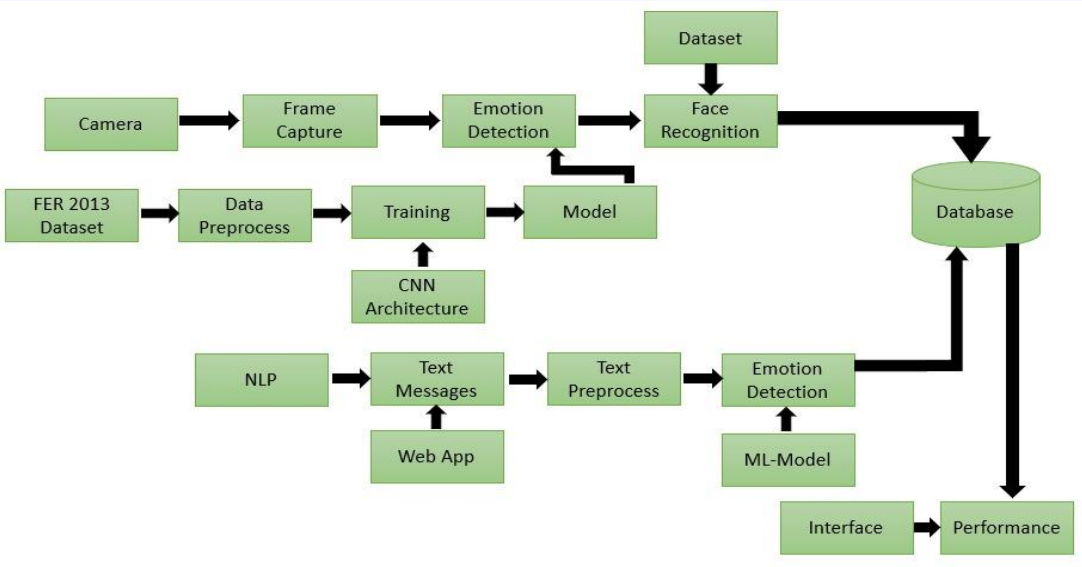
\includegraphics[width=125mm]{basic arch.png}
\caption{Architecture Diagram}
\end{figure} 

\paragraph{}
A face recognition system is a complex technology that uses several components to identify individuals from their facial features. The basic architecture of a face recognition system can be divided into two main stages: feature extraction and face recognition.

\paragraph{}
In the feature extraction stage, the system first detects a face in an image, typically using a deep learning algorithm. Once the face is detected, the system extracts a set of unique features from the face, such as the distance between the eyes, the shape of the nose, and the texture of the skin. These features are then stored in a database.

\paragraph{}
In the face recognition stage, when a new image is presented to the system, the system extracts features from the new face and compares them to the features stored in the database. If there is a match, the system identifies the person in the new image. The accuracy of the face recognition system depends on the quality of the image, the size and diversity of the database, and the effectiveness of the feature extraction and matching algorithms.


\subsection{CNN Architecture}
\paragraph{}
The face recognition process begins with image capture, followed by face detection and preprocessing for normalization. Feature extraction identifies unique facial characteristics, compared against a stored database for identification. Emotion detection assesses emotional states, aided by text preprocessing. The web app acts as the user interface, while the ML model trains algorithms for face recognition and emotion detection. The system's accuracy is evaluated in the performance component.
\begin{figure}[!ht]
\centering
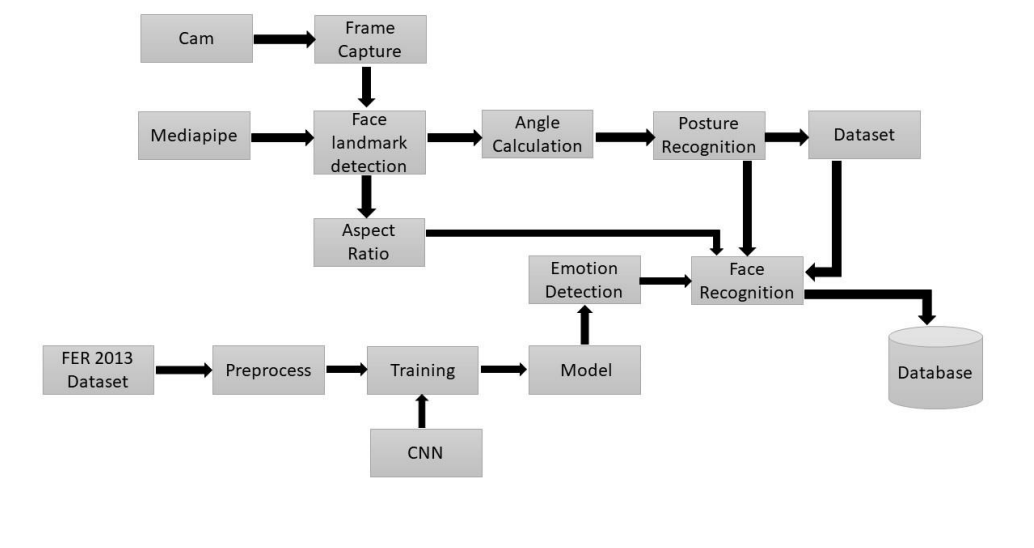
\includegraphics[width=125mm]{cnn arch.png}
\caption{CNN Architecture }
\end{figure}

\subsection{NLP Architecture}
\par \hspace{1cm}The NLP architecture employed in predicting students academic performance typically comprises four key components: text preprocessing, feature extraction, machine learning algorithm, and evaluation. Text preprocessing involves cleaning and preparing the text data, while feature extraction focuses on identifying relevant features from the text. The machine learning algorithm, often a recurrent neural network (RNN), utilizes the extracted features to predict academic performance. Evaluation assesses the model's performance on a held-out test set to prevent overfitting. This intricate architecture enables the prediction of students' academic performance, empowering educators to provide timely interventions for at-risk students.
\begin{figure}[!ht]
\centering
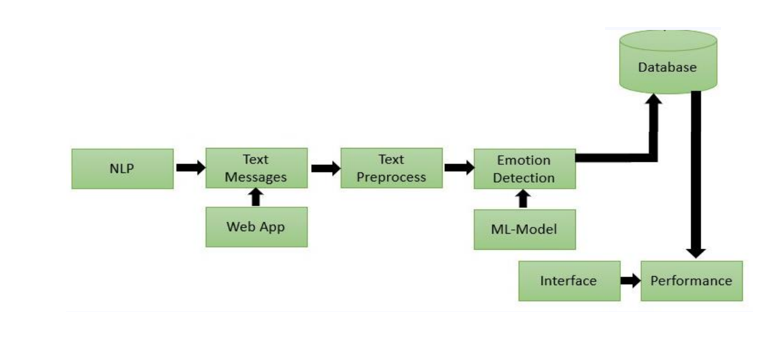
\includegraphics[width=125mm]{archhhh.PNG}
\caption{NLP Architecture}
\end{figure} 

\section{DFD}
\par \hspace{1cm} The data flow diagram is used to define the flow of the system and its resources
such as information. Data flow diagrams are a way of expressing system requirements
in a graphical manner. Data flow diagrams represent one of the most ingenious tools
used for structured analysis. A Data flow diagram or DFD as it is shortly called is
also known as a bubble chart. It has the purpose of clarifying system requirements
and identifying major transformations that will become programs in system design.
It is the major starting point in the design phase that functionally decomposes the
requirement specifications down to the lowest level of details.
A data flow diagram consists of a series of bubbles joined by lines. The bubble
represents data transformation and lines represent flow in the system. In the normal
convention, a Data flow diagram has four major symbols.
\begin{itemize}
    \item Square, defines the source or destination of data.
    \item Arrow, which shows data flow. 
    \item Circle, which represents a process that transforms incoming data into the outgoing flow.
    \item Open rectangle, which shows data store.
\end{itemize}
The Data flow diagram at the simplest level is referred to in simple words as
a “CONTEXT ANALYSIS DIAGRAM”. These are expanded by level, each
explaining its process in detail. Processes are numbered for easy identification
and are normally labeled in block letters. Each data flow is labeled for easy
understanding.
\par • PROCESS: The process shows the work of the system. Each process has one
or more data inputs and produces one or more data outputs. Processes are
represented by round rectangles in the Data flow Diagram. Each process has a
unique name and number. This name and number appear inside the rectangle
that represents the process in a Data flow Diagram. Process names should be
unambiguous and should convey as much meaning as possible without being
too long.
\par • DATASTORES: A datastore is a repository of data. Processes can enter data
into a store or retrieve data from the data store. Each data has a unique name.
\par • DATA FLOWS: Data flows show the passage of data in the system and are
represented by the lines joining system components. An arrow indicates the
direction of flow and the line is labeled by name of the data flow.
\par • EXTERNAL ENTITIES: External entities are outside the system but they can
either supply data into the system or use other systems output. They are entities
on which the designer has control. They may be an organization’s customer or
other bodies with which the system interacts. External entities that supply data
into the systems are sometimes called sources. External entities that use the system data are sometimes called sinks. These are represented by rectangles in
the DFD.

\begin{figure}[!ht]
\centering
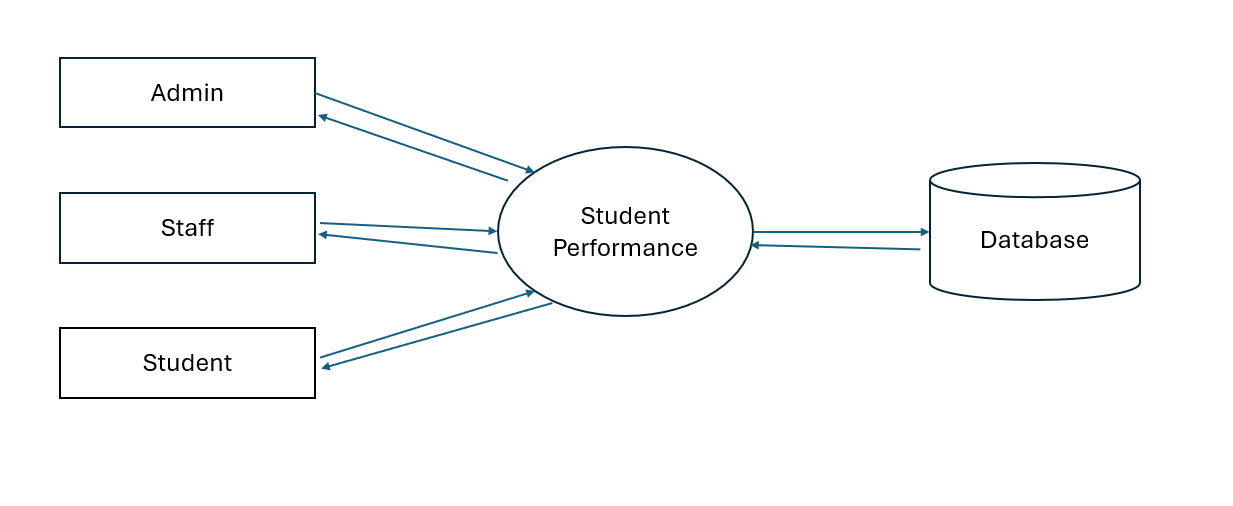
\includegraphics[width=125mm]{dfd.png}
\caption{DFD-Level 0}
\end{figure} 

\begin{figure}[!ht]
\centering
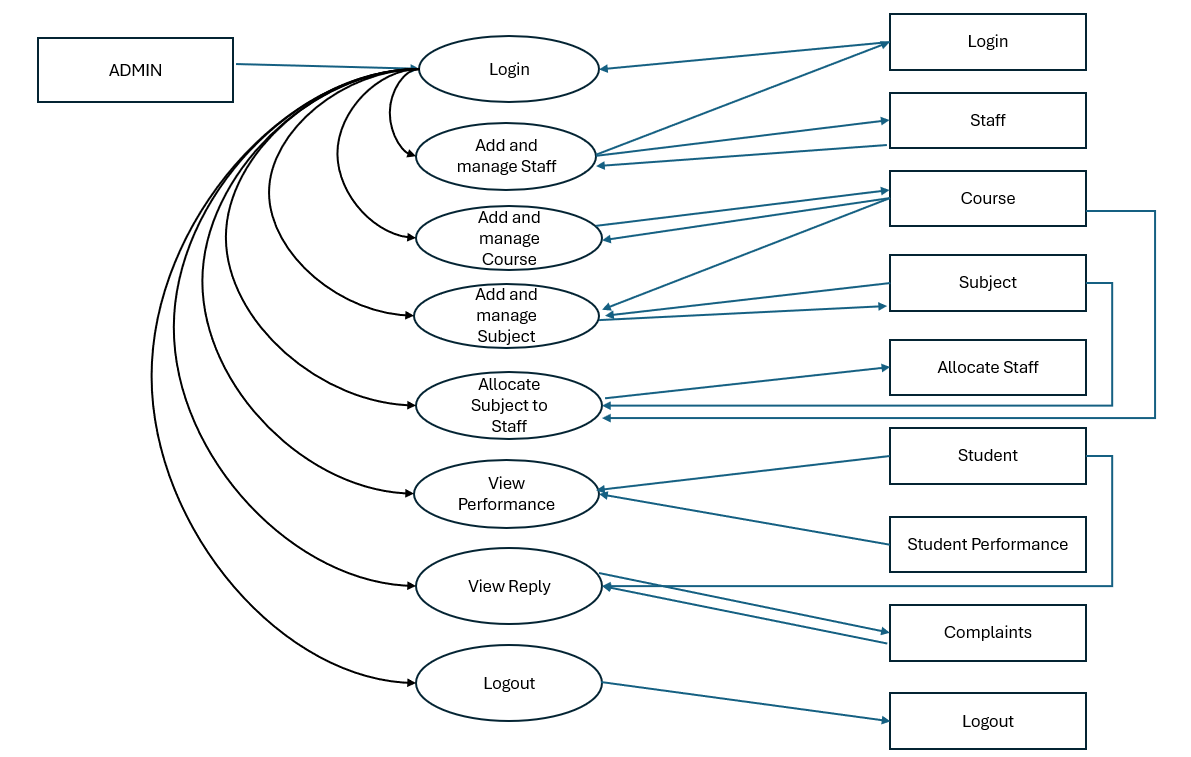
\includegraphics[width=125mm]{admin dfd.png}
\caption{DFD Admin-Level 1.1}
\end{figure} 

\begin{figure}[!ht]
\centering
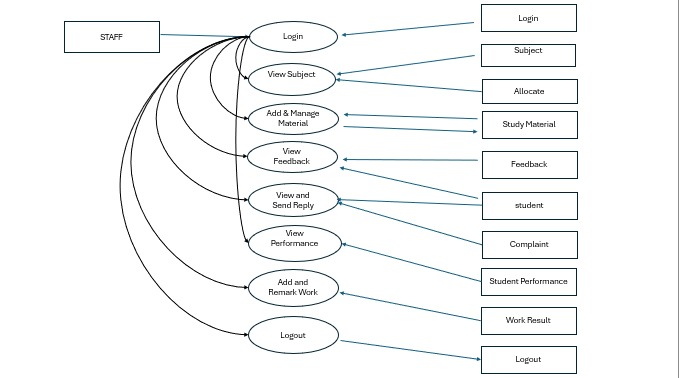
\includegraphics[width=125mm]{WhatsApp Image 2024-04-26 at 1.31.39 AM (1).jpeg}
\caption{DFD Staff-Level 1.2}
\end{figure} 

\begin{figure}[!ht]
\centering
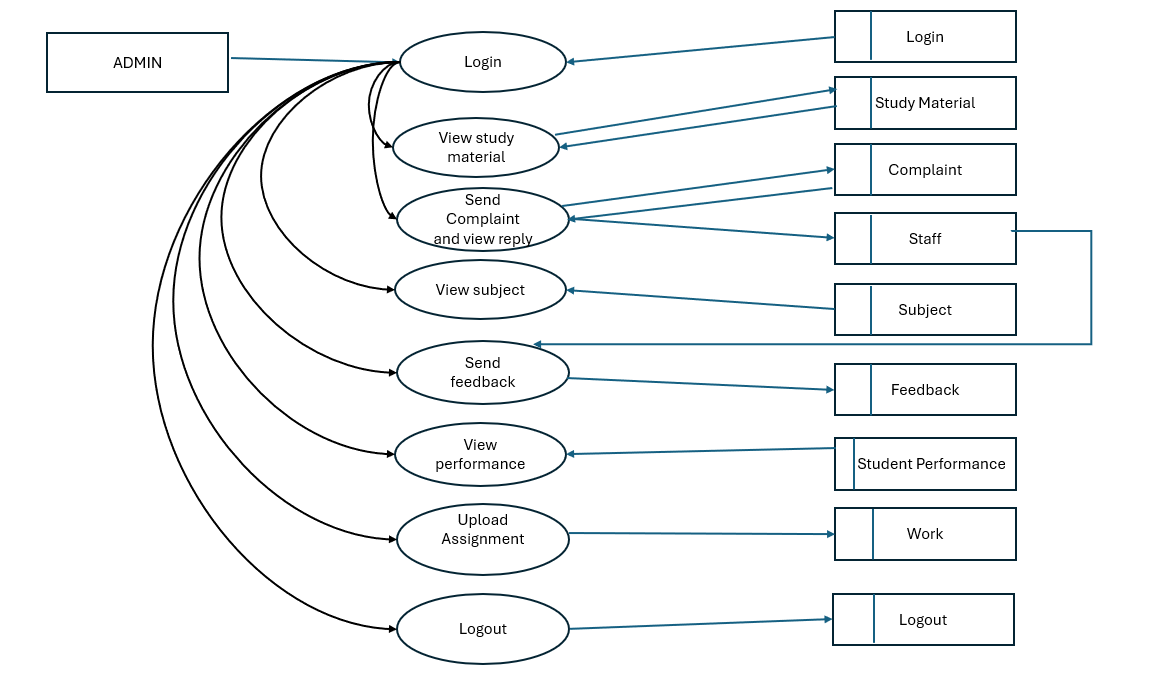
\includegraphics[width=125mm]{student dfd.png}
\caption{DFD Student-Level 1.3}
\end{figure} 



\chapter[IMPLEMENTATION]{\fontsize{16}{12}\vspace{-.59in}\selectfont IMPLEMENTATION}
\section{Algorithms}
\paragraph{}The project utilizes advanced algorithms employing both NLP, Face recoginition, Emotion detection and Posture analysis for effective performance prediction.

\subsection{Emotion classification}
\paragraph{} Emotion classification through facial recognition in evaluating student performance involves using computer vision algorithms to analyze facial expressions and body posture to determine the emotional state and engagement level of a student. The system would use facial recognition algorithms to detect and classify the emotions displayed on the student's face. This could include emotions like happiness, sadness, anger, surprise, and disgust. Machine learning models are trained on labeled facial expression datasets to accurately recognize these emotions. CNNs are used to process visual data from cameras positioned in the classroom or learning environment. These networks can detect and analyze students' body language, gestures, and posture. For instance, slouched posture or frequent yawning may indicate fatigue or disengagement, while active participation and attentive posture suggest involvement and interest. By monitoring students' physical behavior, educators can identify signs of boredom, fatigue, or distraction and intervene appropriately to re-engage students.

\subsection{Posture Analysis}
\paragraph{} By analyzing the student's body posture, the system can assess their level of engagement and alertness. Slouched posture or leaning too far back might indicate disengagement or tiredness, while an upright posture may suggest attentiveness. MediaPipe is used in Eye Angle Monitoring the angle of the student's eyes and can help detect signs of drowsiness or fatigue. For example, if the eyes are closed or nearly closed for an extended period, it may indicate that the student is falling asleep or not paying attention.

\subsection{NLP}
\paragraph{} Natural Language Processing (NLP) combined with facial recognition and Convolutional Neural Networks (CNNs) presents a powerful tool for academic performance evaluation of students. This innovative approach leverages machine learning and computer vision techniques to provide a comprehensive analysis of a student's performance, engagement, and comprehension during educational activities.

\par NLP techniques are used to analyze textual data such as written responses, essays, or transcriptions of verbal answers. Sentiment analysis can gauge the emotional tone of the text, detecting signs of confusion, frustration, or confidence. Furthermore, semantic analysis can assess the depth of understanding by examining the coherence and relevance of the content to the given topic. By analyzing text responses, educators can gain insights into students' comprehension levels, critical thinking abilities, and emotional responses to academic material.

\par The data from text analysis, facial recognition, and CNNs are integrated and analyzed to provide a holistic evaluation of students' academic performance. Machine learning algorithms combine these data sources to generate personalized insights and recommendations for each student. For example, if a student consistently exhibits signs of confusion in text responses and facial expressions, the system may suggest additional explanations, practice exercises, or one-on-one tutoring sessions to address the underlying challenges.

\par In conclusion, NLP combined with facial recognition and CNNs offers a sophisticated tool for academic performance evaluation, allowing educators to gain valuable insights into students' comprehension, engagement, and emotional states. By leveraging these technologies, educators can create more personalized learning experiences, support struggling students, and foster a positive and inclusive educational environment.


\section{Web Applications}
\paragraph{} Web applications are created using HTML, CSS and JavaScript. In this project, initially the web pages are created for admin, staff and student including their sub pages. Then, they are styled using CSS and various functionalities are added using JavaScript. After its creation, these are connected using Python Framework Django. In Django, we create different routes for each web pages and rendered with route calls. System uses SQLyog server as back-end and communicates with SQL queries.

\subsection{FRONT END}
\subsubsection{HTML}
\paragraph{} The HyperText Markup Language or HTML is the standard markup language for documents designed to be displayed in a web browser. Web browsers receive HTML documents from a web server or from local storage and render the documents into multimedia web pages. HTML describes the structure of a web page semanti- cally and originally included cues for the appearance of the document. HTML ele- ments are the building blocks of HTML pages. With HTML constructs, images and other objects such as interactive forms may be embedded into the rendered page. HTML provides a means to create structured documents by denoting structural se- mantics for text such as headings, paragraphs, lists, links, quotes, and other items.
\subsubsection{CSS}
\paragraph{} Cascading Style Sheets (CSS) is a style sheet language used for describing the presentation of a document written in a markup language such as HTML.CSS is a cor- nerstone technology of the World Wide Web, alongside HTML and JavaScript.CSS is designed to enable the separation of presentation and content, including layout, colors, and fonts. This separation can improve content accessibility, provide more flexibility and control in the specification of presentation characteristics, enable mul- tiple web pages to share formatting by specifying the relevant CSS in a separate .css file which reduces complexity and repetition in the structural content as well as enabling the .css file to be cached to improve the page load speed between the pages that share the file and its for- matting. Separation of formatting and content also makes it feasible to present the same markup page in different styles for different rendering methods, such as on-screen, in print, by voice (via speech-based browser or screen reader), and on Braille-based tactile devices.

\subsubsection{JavaScript}
\paragraph{} JavaScript often abbreviated as JS, is a programming language that conforms to the ECMAScript specification. JavaScript is high-level, often just-in-time compiled, and multi-paradigm. It has curly-bracket syntax, dynamic typing, prototype-based object- orientation, and first-class functions.JavaScript is one of the core technologies of the World Wide Web.

\subsubsection{Bootsrtap}
\paragraph{}JavaScript often abbreviated as JS, is a programming language that conforms to the ECMAScript specification. JavaScript is high-level, often just-in-time compiled, and multi-paradigm. It has curly-bracket syntax, dynamic typing, prototype-based object- orientation, and first-class functions.JavaScript is one of the core technologies of the World Wide Web.

\subsection{BACK END}
\subsubsection{Python}
\paragraph{}Python is a general-purpose interpreted, interactive, object-oriented, and high- level programming language. Python is a high-level, interpreted, interactive and object-oriented scripting language. Python is designed to be highly readable. It uses English keywords frequently whereas other languages use punctuation, and it has fewer syntactical constructions than other languages. Python is Interpreted Python is processed at run-time by the interpreter. Users do not need to compile the pro- gram before executing it. This is similar to PERL and PHP. Python is an Interactive User who can sit at a Python prompt and interact with the interpreter directly to write programs. Python is Object-Oriented Python supports Object-Oriented style or technique of programming that encapsulates code within objects. Python is a Be- ginner’s Language Python is a great language for beginner-level programmers and supports the development of a wide range of applications from simple text process- ing to WWW browsers to games.

\subsubsection{MySQL}
\paragraph{} MySQL is an open-source relational database management system(RDBMS). Its name is a combination of ”My”, the name of co-founder Michael Widenius’s daughter, and ”SQL”, the abbreviation for Structured Query Language. A relational database organizes data into one or more data tables in which data types may be related to each other; these relations help structure the data. SQL is a language pro- grammers use to create, modify and extract data from the relational database, as well as control user access to the database. In addition to relational databases and SQL,
an RDBMS like MySQL works with an operating system to implement a relational database in a computer’s storage system, manages users, allows for network access, and facilitates testing database integrity and creation of backups.MySQL is free and open-source software under the terms of the GNU General Public License and is also available under a variety of proprietary licenses. MySQL was owned and sponsored by the Swedish company MySQL AB, which was bought by Sun Micro-systems.

\subsubsection{Django}
\paragraph{} Django is a high-level Python web framework that simplifies the process of building web applications by providing a robust set of tools and features. Django includes features such as an Object-Relational Mapping (ORM) layer for database interaction, a URL routing system, a templating engine, and a built-in administrative interface. developers can quickly create database-driven websites or web applications by focusing on writing Python code rather than dealing with repetitive tasks like database management or user authentication. Its design promotes clean and maintainable code, making it popular among developers for projects of all sizes, from simple websites to complex web applications.


\section{Desktop Application}
\paragraph{} The Desktop Application is developed using the Python programming language within the PyCharm IDE. It utilizes a combination of NLP and facial emotion detection to evaluate academic performance.

\par Using Python libraries such as TensorFlow, Keras, OpenCV, NumPy, Pandas, and the Facial Expression Recognition Dataset, the application generates a model for facial emotion recognition. The FER-2013 dataset, available on Kaggle, contains grayscale images of faces with corresponding emotion labels. The dataset includes seven emotions: Angry, Disgust, Fear, Happy, Sad, Surprise, and Neutral. For academic performance evaluation, Happy, Surprise, and Neutral are considered positive responses, while Angry, Disgust, Fear, and Sad are considered negative responses.

\par In this context, a deep CNN model is fed with the facial expressions of students, allowing the system to recognize emotional responses during learning activities. The coursework provided to students judges their performance ,along with their facial recognition.

\par Through the integration of NLP and facial emotion detection, this Desktop Application offers a dynamic and personalized approach to academic performance evaluation. By analyzing students' emotional responses and providing coursework, educators can optimize learning experiences, foster engagement, and improve overall academic outcomes for students.



\section{Screenshots}
\subsection{Login Form}
\paragraph{} Fig. 5.1 shows the login page of the project, which uses a username and password for authentication and also offers an option for student registration.
\begin{figure}[!ht]
\centering
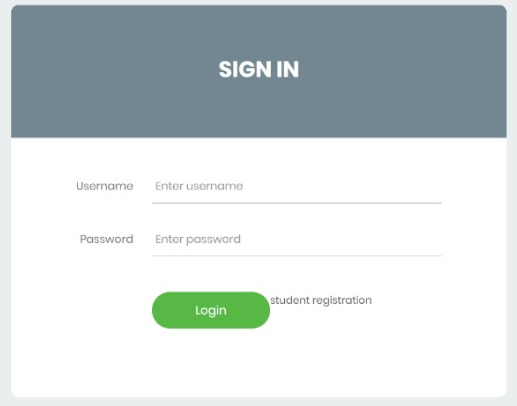
\includegraphics[width=125mm]{login.png}
\caption{Login Form}
\end{figure} 

\subsection{Admin-Home Page}
\paragraph{} Fig. 5.2 depicts the admin home page, displaying options for managing various functionalities.

\begin{figure}[!ht]
\centering
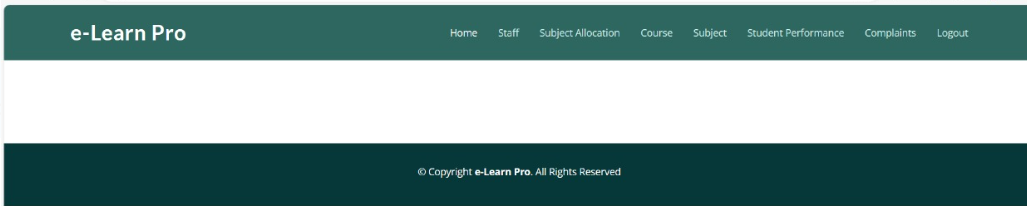
\includegraphics[width=125mm]{Admin homepage.png}
\caption{Admin-Home Page}
\end{figure} 

\subsection{Staff-Home Page}

\paragraph{} Fig. 5.3 depicts the staff homepage, which likely provides educators with a central hub for monitoring student performance. The interface offer functionalities student information panels, potentially allowing educators to assess student progress and identify areas needing attention.
\begin{figure}[!ht]
\centering
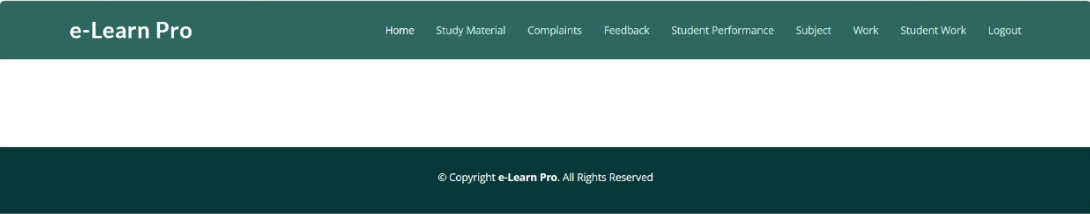
\includegraphics[width=125mm]{staff homepage.png}
\caption{Staff-Home Page}
\end{figure} 

\subsection{Student-Home Page}
\paragraph{} Fig. 5.4 shows the student homepage, potentially offering a personalized view of academic performance with feedback and resources tailored to individual needs.
\begin{figure}[!ht]
\centering

\includegraphics[width=125mm]{student homepage.png}
\caption{Student-Home Page}
\end{figure} 

\subsection{Emotion Detection And Posture Analysis}
\paragraph{} Fig. 5.5 depicts a potential interface for face recognition and emotion detection system, which are typically designed to analyze student faces in a video stream and potentially infer emotions.Fig. 5.6 hint at a functionality for posture analysis. This system could analyze student posture to potentially gauge their alertness level during lectures.

\begin{figure}[!ht]
\centering
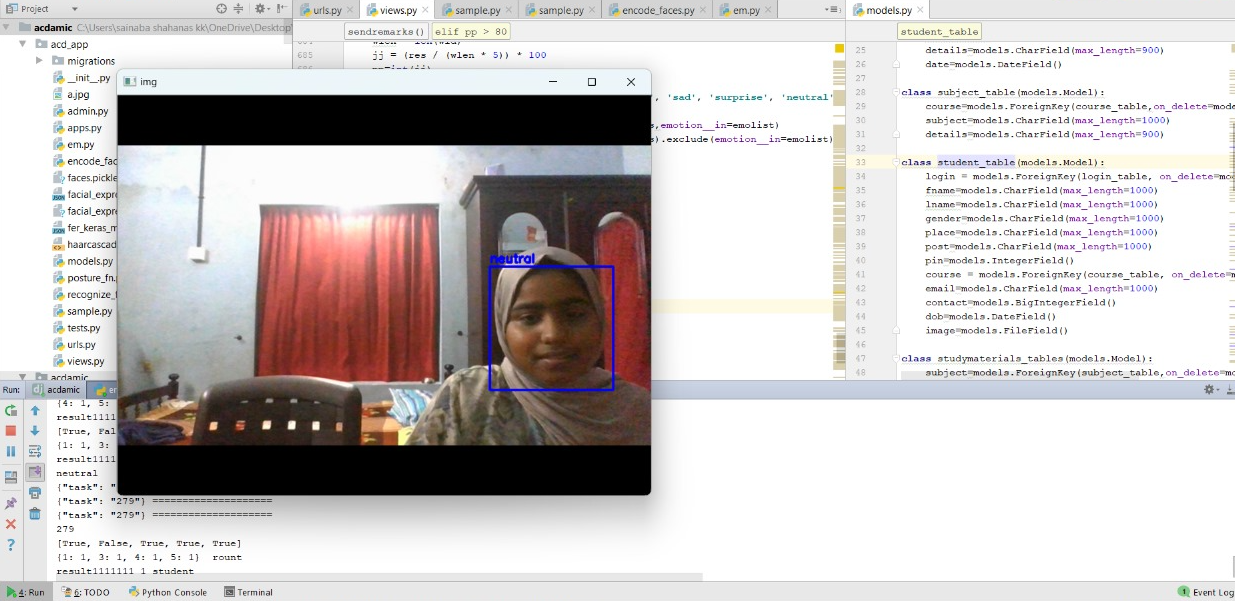
\includegraphics[width=125mm]{emotion detection and facial recognition.png}
\caption{Emotion Detection And Facial Recognition}
\end{figure} 


\begin{figure}[!ht]
\centering
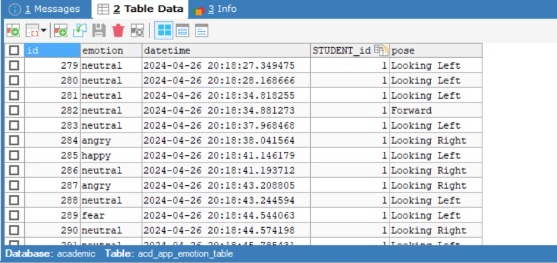
\includegraphics[width=125mm]{post database.png}
\caption{Posture Database}
\end{figure} 

\subsection{Performance Measure}

\paragraph{} Fig. 5.7 an upload option is given to upload assignments to the student to check whether the student is performing well or not.Fig. 5.9 depicts that the staff can remark the respective work uploaded by student and thus resulting in prediction
\begin{figure}[!ht]
\centering
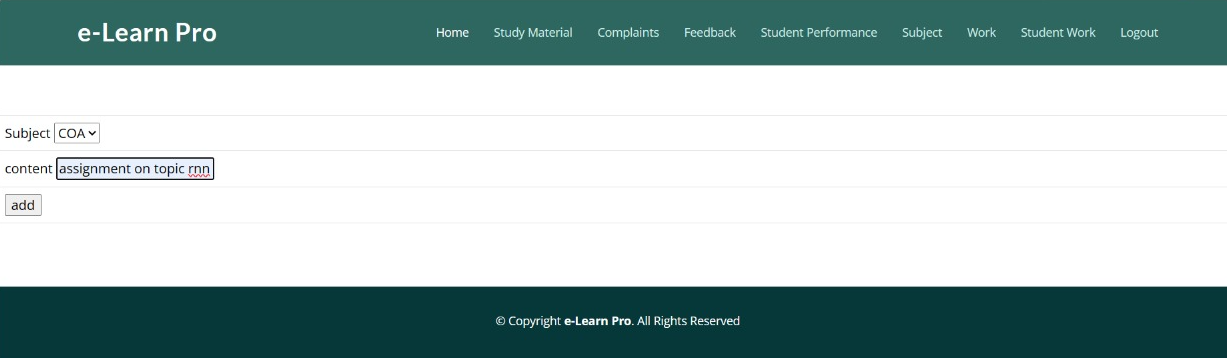
\includegraphics[width=125mm]{staff assigning wo.png}
\caption{NLP: Staff Assigning Work}
\end{figure} 

\begin{figure}[!ht]
\centering
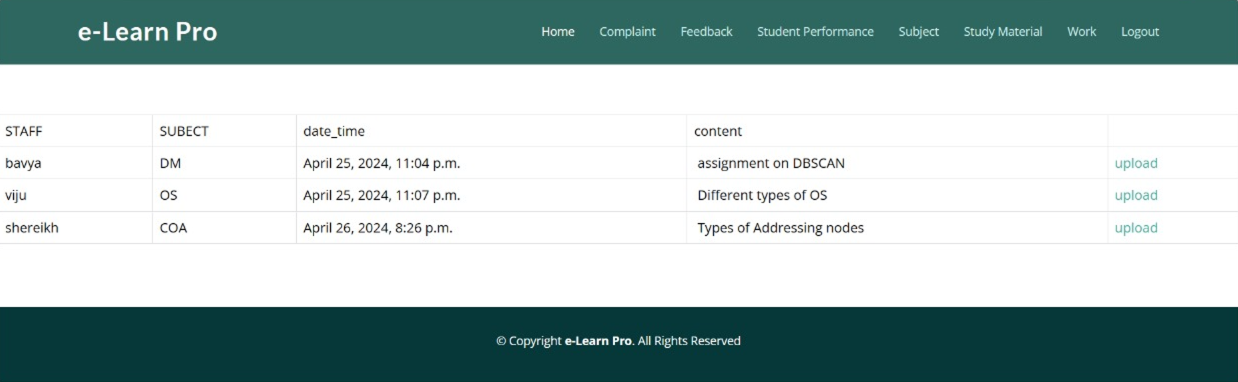
\includegraphics[width=125mm]{student uplooad .png}
\caption{Student Upload Work}
\end{figure} 


\begin{figure}[!ht]
\centering
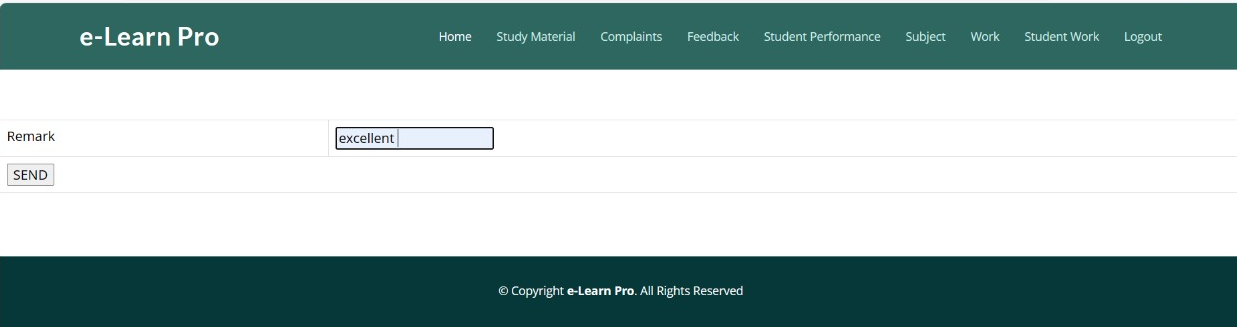
\includegraphics[width=125mm]{remarks by staff.png}
\caption{Remarks By Staff}
\end{figure} 




\chapter[RESULT ANALYSIS]{\fontsize{16}{12}\vspace{-.59in}\selectfont RESULT ANALYSIS}

\section{Output}

\paragraph{} The project explored the potential of combining Natural Language Processing with facial recognition, posture analysis, and emotion detection to predict student performance. This multifaceted approach aimed to provide educators with a richer understanding of student comprehension, engagement, and emotional state. 

The results of the project are promising. By analyzing student text data (e.g., essays, responses), facial expressions, posture, and potential emotions, the model was able to predict academic performance with a certain degree of accuracy. This allowed for early identification of students who might be struggling or disengaged, enabling educators to tailor their teaching strategies and provide targeted support. 


\begin{itemize}
    \item Face recognition and emotion detection: It utilizes machine learning within the OpenCV library. This allows for advanced face detection, potentially using a Deep Neural Network model for superior accuracy. Once a face is identified, additional processing might involve a Haar cascade classifier for basic verification or emotion recognition. However, for deeper emotional analysis, the system likely leverages a separate pre-trained model within OpenCV to provide more nuanced insights.
    \item Posture Analysis: It utilizes MediaPipe's Pose Landmarker to analyze student posture in videos or images. This allows us to assess engagement and alertness by tracking body landmarks and potentially eye gaze direction. By analyzing posture, we can identify signs of disinterest, fatigue, or drowsiness, providing valuable insights for educators.
    \item NLP: Project utilizes NLP techniques to analyze student-written text (essays, responses) and transcribed speech. This analysis goes beyond comprehension, using sentiment analysis to gauge student emotions like frustration or confidence. It leverage NLTK, a Python library for NLP tasks, to process text and potentially use pre-trained models for tasks like sentiment analysis. NLP is also applied to analyze staff remarks, providing a broader perspective for predicting student performance.

\end{itemize}

\begin{figure}[!ht]
\centering
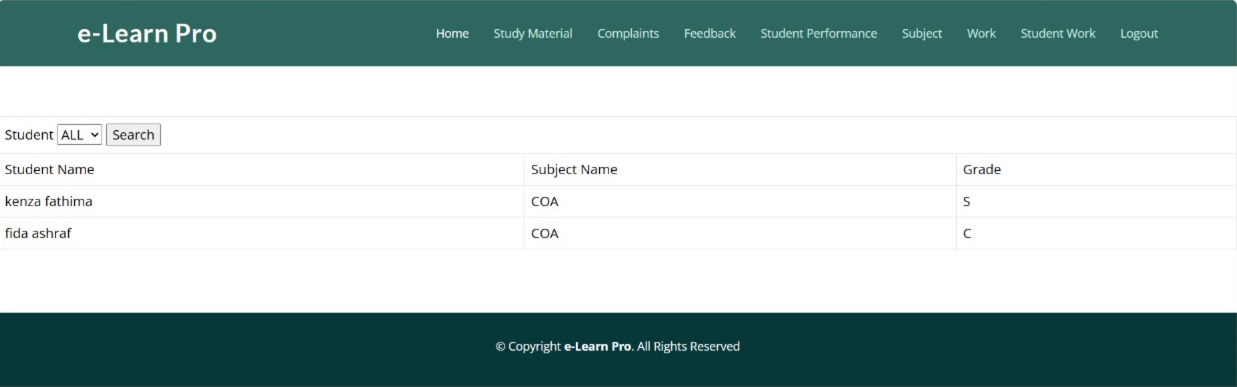
\includegraphics[width=125mm]{prediction and performance .png}
\caption{NLP:Prediction Of Performance}
\end{figure} 


\section{Comparison}
\paragraph{} Comparison highlights how our project offers a broader and potentially more insightful approach to academic performance prediction compared to Zhen et al. (2023).[1]

\begin{figure}[!ht]
\centering
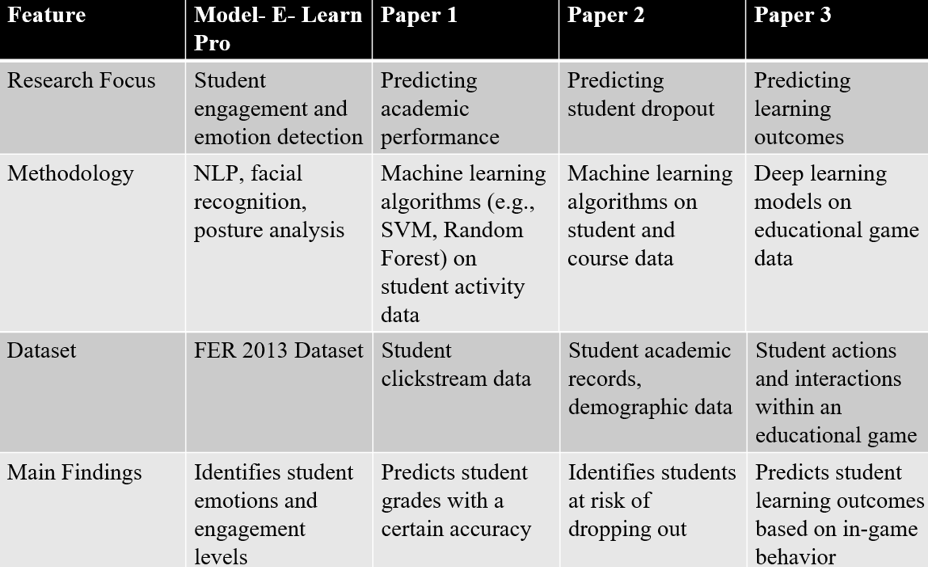
\includegraphics[width=125mm]{ss final.png}
\caption{Comparison}
\end{figure} 

\paragraph{} \textbf{Focus:} Both projects utilize NLP techniques. However, our project expands on Zhen et al.'s focus on online interactions by incorporating face recognition, emotion detection, and posture analysis. This allows us to capture a more holistic view of student engagement and well-being beyond just textual communication.

\paragraph{} \textbf{Data Analysis:}  While Zhen et al. analyze student dialogue in online classes, our project leverages a richer dataset that includes student text analysis (essays, responses), facial expressions, body language, and potential emotions. This offers a more multifaceted perspective on student learning.
\paragraph{} \textbf{Applicability:}  Our project is designed to work in traditional classroom settings, expanding its applicability beyond the online environment studied by Zhen et al. (2023).[1]

\paragraph{} \textbf{Insights:} Both projects aim to predict academic performance. However, our real-time analysis of emotions, engagement, and posture might offer additional insights for immediate intervention and personalized learning strategies.

\paragraph{} Overall, our project builds upon Zhen et al.'s (2023) work by offering a broader range of data analysis techniques and wider applicability.[1]

\section{Performance Evaluation}
\paragraph{} Model's performance is evaluated using a classification report and confusion matrix. This report analyzes how well the model predicts student performance categories using precision, recall, and F1-score.Precision measures the accuracy of positive predictions. Recall identifies how well the model finds all positive cases, and F1-score balances these for a comprehensive view.


\begin{figure}[!ht]
\centering
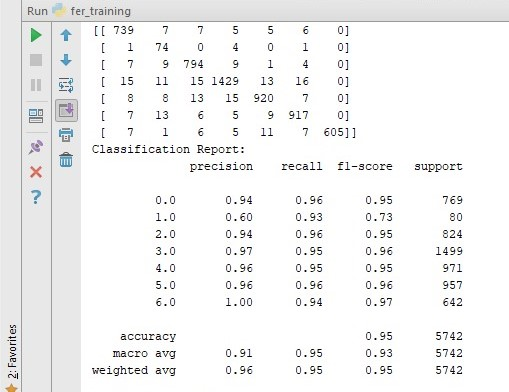
\includegraphics[width=125mm]{e learn .jpeg}
\caption{Classification Report Of E-Learn Pro}
\end{figure} 



\begin{figure}[!ht]
\centering
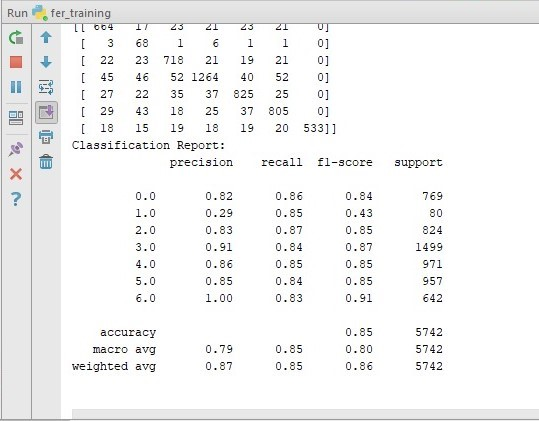
\includegraphics[width=125mm]{rnn.jpeg}
\caption{Classification Report Of RNN Model}
\end{figure} 

\begin{figure}[!ht]
\centering
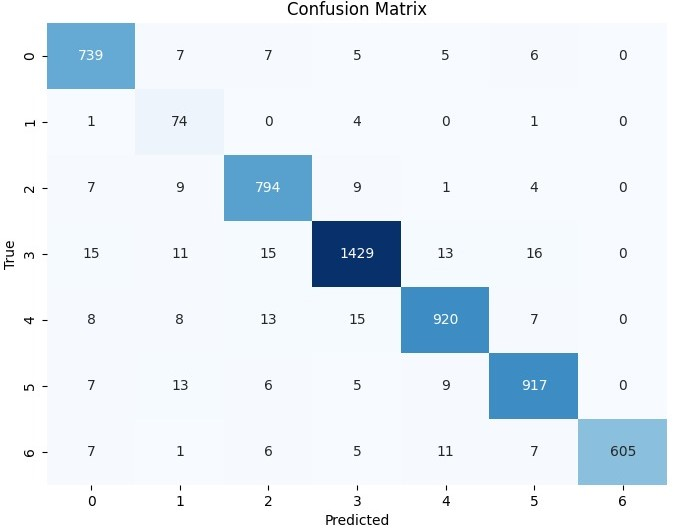
\includegraphics[width=125mm]{e learn conf.jpeg}
\caption{Confusion Matrix Of E-Learn Pro}
\end{figure} 

\begin{figure}[!ht]
\centering
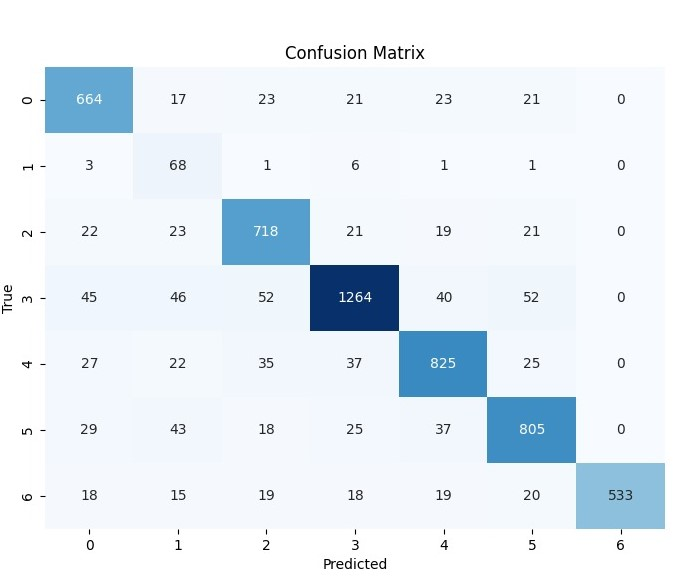
\includegraphics[width=125mm]{rnn conf.jpeg}
\caption{Confusion Matrix Of RNN Model}
\end{figure} 

\paragraph{} The model achieved an accuracy of 95\% in predicting student performance and demonstrated a 10\% improvement in accuracy compared to existing models, suggesting a better ability to identify struggling students.



\chapter[CONCLUSION AND FUTURE WORK]
{\fontsize{16}{12}\vspace{-.59in}\selectfont CONCLUSION AND FUTURE WORK}
\par \hspace{1cm}In conclusion, this research explores the intricate relationship between classroom dialogue and the academic performance of students in primary school, specifically focusing on live classroom interactions. Leveraging automated text classification models based on natural language processing techniques, the study identifies interaction features and assesses their predictive power for academic performance.
\par Notably, this distinguishes between non-stem and stem courses, uncovering nuanced patterns in emotional expression and interactive types. The findings emphasize the significance of interactive dialogue in integrating knowledge building and social interaction. Importantly, the study establishes prediction models, revealing that interactive features play a more crucial role in stem courses. 
\par It provides practical insights for educators, online education platforms, and policymakers, highlighting the need for tailored teaching strategies, support mechanisms, and course evaluations based on the unique characteristics of non-stem and stem courses. However, the study acknowledges limitations, such as the potential imprecision in stage divisions and the necessity for fine-grained analyses. Future research should explore diverse learning contexts, incorporate additional data modalities, and delve into causal relationships to further enhance our understanding of live classroom prediction dynamics.
 \par To enhance predictive models, there is a need for fine-tuning interaction features extracted from live classroom data, delving into nuanced elements within emotional expression, interactive types, and interaction frequencies. A more dynamic and adaptive analysis of classroom stages, considering actual teaching time and evolving student-teacher interactions, could provide a more accurate representation of the learning process. Cross-cultural validation is crucial to determine the generalizability of findings across diverse educational settings globally. Incorporating multimodal data, such as video, audio, and physiological signals, can offer a comprehensive understanding of student experiences.
 \par Future research should move beyond correlation to explore causal relationships between interaction features and academic performance, enabling the development of targeted intervention strategies. Exploring the applicability of findings in different learning environments, conducting longitudinal studies, and continuously validating predictive models are essential steps toward refining our understanding of the intricate interplay between live classroom interactions and student outcomes. These endeavors collectively contribute to a more robust, adaptable, and universally applicable framework for predicting and enhancing academic performance based on real-time classroom dynamics.




